%Sample Headers:
%Introduction and objectives
%Background information and previous work in the subject area (referenced)
%Theoretical aspects/modelling/simulation/strategies
%Experimental techniques/methods/apparatus/rationale
%Results
%Discussion of results/critical analysis/comparison with other work
%Suggestions for future work
%Conclusions
%References
%Appendices (equations/program code/equipment specifications)
%Logbook (for Teaching Periods 1 and 2 – ensure there is an entry for every week)

\chapter{Introduction and Objectives}

This project is focused on examining the effects of non-deterministic timing error in digital amplitude-modulation radio signal receivers. Timing errors remain an important issue in modern digital receivers, despite considerable research into improved clock generation and recovery circuits. This project takes a novel approach to the problem, as instead of trying to reduce the level of timing error, it assumes statistical knowledge of the timing error present and attempts to mitigate its effects at the decoding stage.

Work was divided into two parts:

\begin{itemize}
\item
The effects of timing error on the received signal at the input to the decoder were examined, in order to determine the probability density function seen by the decoder.
\item
Using knowledge of the nature of the signal at the input of the decoder, communications theory was used to determine the optimum decoder for the given signal.
\end{itemize}

The ultimate goal was to demonstrate an optimum decoder that would perform significantly better than traditional decoders designed assuming perfect timing synchronisation. Numerical simulation work was backed up with a mathematical analysis.

\chapter{Background Information}

\section{The Communications system Model}

A typical radio communications system consists of a transmitter, a
receiver and a communications channel, that may contain any number of
non-idealities typically caused by stochastic processes. By modeling these non-idealities using fitting statistical probability distributions, a statistical description of the received signal can be derived and used to inform correct design of the receiver.

One could imagine a binary transmission system that sends one of two
possible signals: a 1V$_{RMS}$ wave if a `0' is to be sent, and a
3V$_{RMS}$ if a `1' is to be sent. After being distorted by the
communications channel, the receiver could in theory see a signal of any
amplitude, and must make a decision as to which amplitude was originally
sent. It would be helpful for the designer to know the probability density function (PDF)
of the received signal, ie. the probability of receiving a signal
amplitude if a known amplitude was sent. If one assumes the communications
channel is memoryless and distorts the signal by adding zero-mean white Gaussian noise,
the received signal PDF will be a Gaussian distribution centred on the
sent signal amplitude, as shown below. If both symbols are equiprobable, their PDF's will be of equal height, and therefore shifted copies of each other.

\begin{figure}[htbp]
\centering
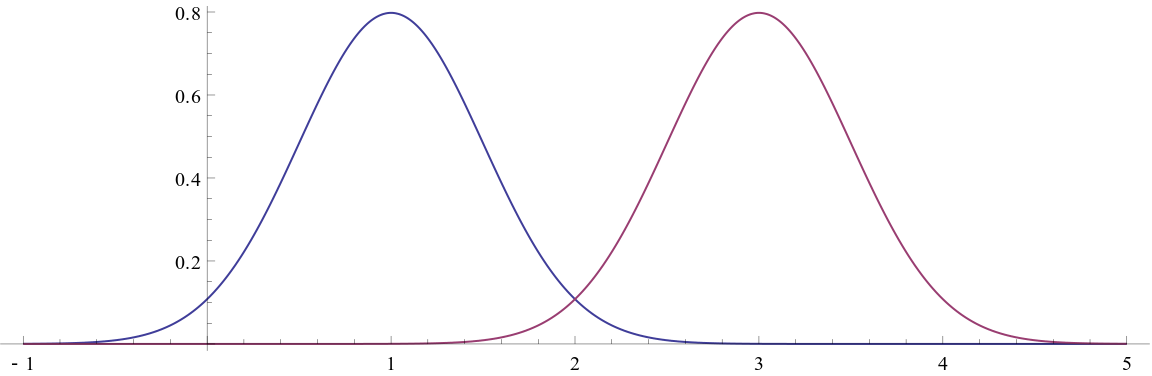
\includegraphics[width=\linewidth]{4-PAM_PDF.png}
\caption[Ideal received signal PDF]{Gaussian noise corrupts a sent signal, resulting in a
probability density function for each possible sent symbol}
\end{figure}

\begin{figure}[htbp]
\centering
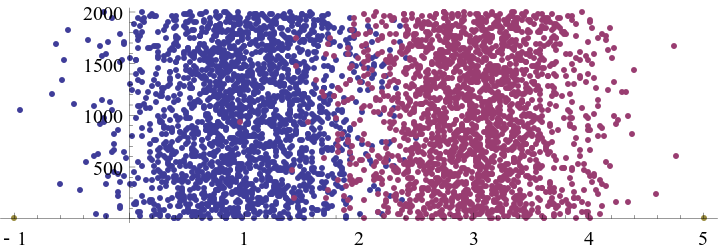
\includegraphics[width=\linewidth]{4-PAM_samples.png}
\caption[AWGN channel simulation]{As an example, 2000 of each symbol has been send down the communications channel. The received values distorted by noise are
plotted above. Note the overlap in received values corresponding to both
symbols: it is impossible to detect the signal with 100\% accuracy.}
\end{figure}

A \emph{maximum-likelihood (ML) detector} seeks to minimise the probability of
error by always picking whichever signal was most likely to be sent, given
the received signal. The derived probability distributions can give us this information. The threshold between picking one value or the other
will be where both symbols are equally likely to be sent, the point of
intersection of both PDF's. Since the Gaussian distribution is symmetric
about its mean, in this case the threshold (or \emph{Decision Region
Boundary}) is exactly midway between both sent amplitudes. Intuitively
this makes sense: it says that in the simplest case if one receives a particular
signal, one should assume whichever possible sent signal is nearest. However in more complicated cases picking the point of intersection of both PDF's
is the more general solution. 

While applicable to cable channels, radio systems have to deal with numerous reflections from the environment, known as fading effects. A superposition of reflected signals, with different levels of attenuation, is therefore seen at the receiver. Traditional communications theory models fading as a random gain. Performance in this case can be improved by capturing multiple signals using multiple antennae, and combining these signals, either using equal weighting (Equal-Gain Combining), or by weighting each channel by its channel gain (Maximal-Ratio Combining).

\section{Transmitter-Receiver Synchronisation}

One issue that complicates detection is \emph{inter-symbol
interference} (ISI). It is possible for signals representing symbols in
the future or past to bleed into the current symbol clock period,
distorting the signal further. For this reason transmitters and receivers
are designed with filtering that applies a \emph{raised cosine function} to the signal.
This filter passes the signal at exactly the symbol's sample time, and attenuates
completely at every other symbol's sample time, ie. at every interval of
$T_{clk}$ for $T \neq 0$. If both receiver and transmitter are perfectly
synchronised, this ensures that the receiver will only see signals
corresponding to the current transmitted symbol, after distortion via
the communications channel.

\begin{figure}[htbp]
\centering
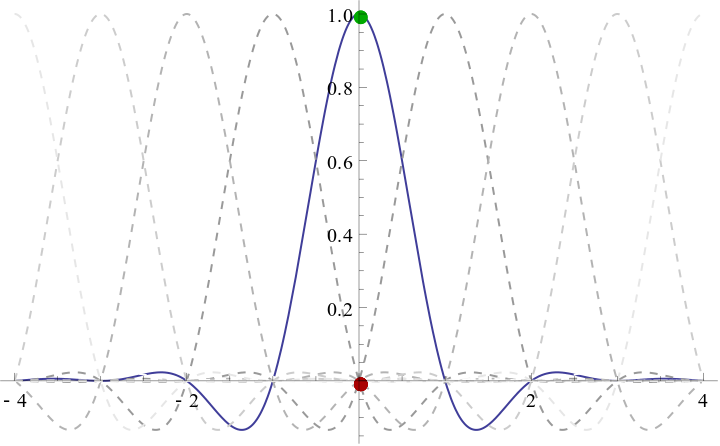
\includegraphics[width=\linewidth]{rrc_sync.png}
\caption[Synchronized raised-cosine response]{A filter with a root raised cosine function is often used, as
it evaluates to 1 at the current sample time and 0 at all other sample
times}
\end{figure}

\begin{figure}[htbp]
\centering
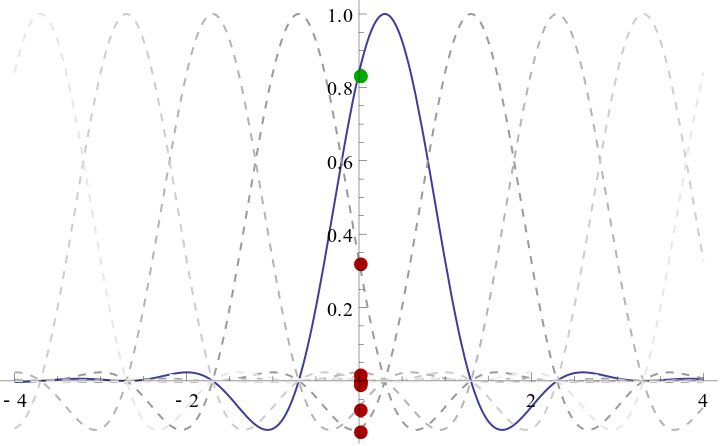
\includegraphics[width=\linewidth]{rrc_err.png}
\caption[Unsynchronized raised-cosine response]{If a timing offset is added to the root raised cosine it no
longer evaluates to 0 or 1 at the sampling time. This results in
reduced receiver performance when the receiver and transmitter are not
properly synchronised.}
\end{figure}

If the receiver and the transmitter are poorly synchronised, however,
the root cosine filter response is shifted in time with respect to the
receiver; adjacent symbols bleed into the current symbol, and the current symbol is attenuated according to the raised cosine function of the timing error. This last point is crucial to this project:

\begin{propo}
An amplitude-modulated system with a given channel function $g[t]$ and a timing error $\delta t$ will experience an attenuation due to the timing error of the transmitted symbol equal to $g[\delta t]$.
\end{propo}

In practice, the adjacent symbols can be modelled as Gaussian noise, and we can therefore express the effects of timing error as a gain dependent on the instantaneous timing error. 

\section{Previous Work}


\chapter{Methodology}

This project models channel noise as additive and Gaussian. Fading is assumed to be Rayleigh-distributed and Maximal-Ratio Combining is considered as a counter-measure (Equal-Gain Combining was examined and found to perform too poorly to be of interest). Timing error is assumed to be Tikhonov-distributed, and knowledge of both channel gain and approximate timing error variance is assumed to be available to the decoder.

A simplified model of a communications system ignoring fading was developed in order to allow the author to familiarise himself with the problem, its associated theory and the \emph{Mathematica} environment. This model was used to verify Proposition 1 above.

the ultimate goal was to prove the existence of sub-optimal performance in the system due to receiver timing errors, and demonstrate an optimum decoder with better performance than traditional decoders assuming perfect synchronisation. The effects of fading were incorporated into the model and the performance of the system in the presence of timing error was examined thoroughly through simulation, to determine the qualitative effects of timing error. The optimum decision region boundaries were then determined to inform the optimum decoder description. Finally, the resulting SER for both receivers was determined from the simulation results.

An analytical verification of these results was attempted by approximating the received symbol PDF conditioned on know timing offsets and channel gains by a Gram-Charlier series and averaging over the respective distributions.

\chapter{Results}

\section{Effects of timing error on the non-fading system}

The general effects of timing error were examined through simulation. A Mathematica simulation of the AWGN communications system with a variable timing error parameter was constructed, and run for a range of timing error parameters.

Timing error was found to result in attenuation of the received signal The level of attenuation depends on the severity of the timing error and the response of the channel, as given be Proposition 1 given earlier.

\begin{figure}[htbp]
\centering
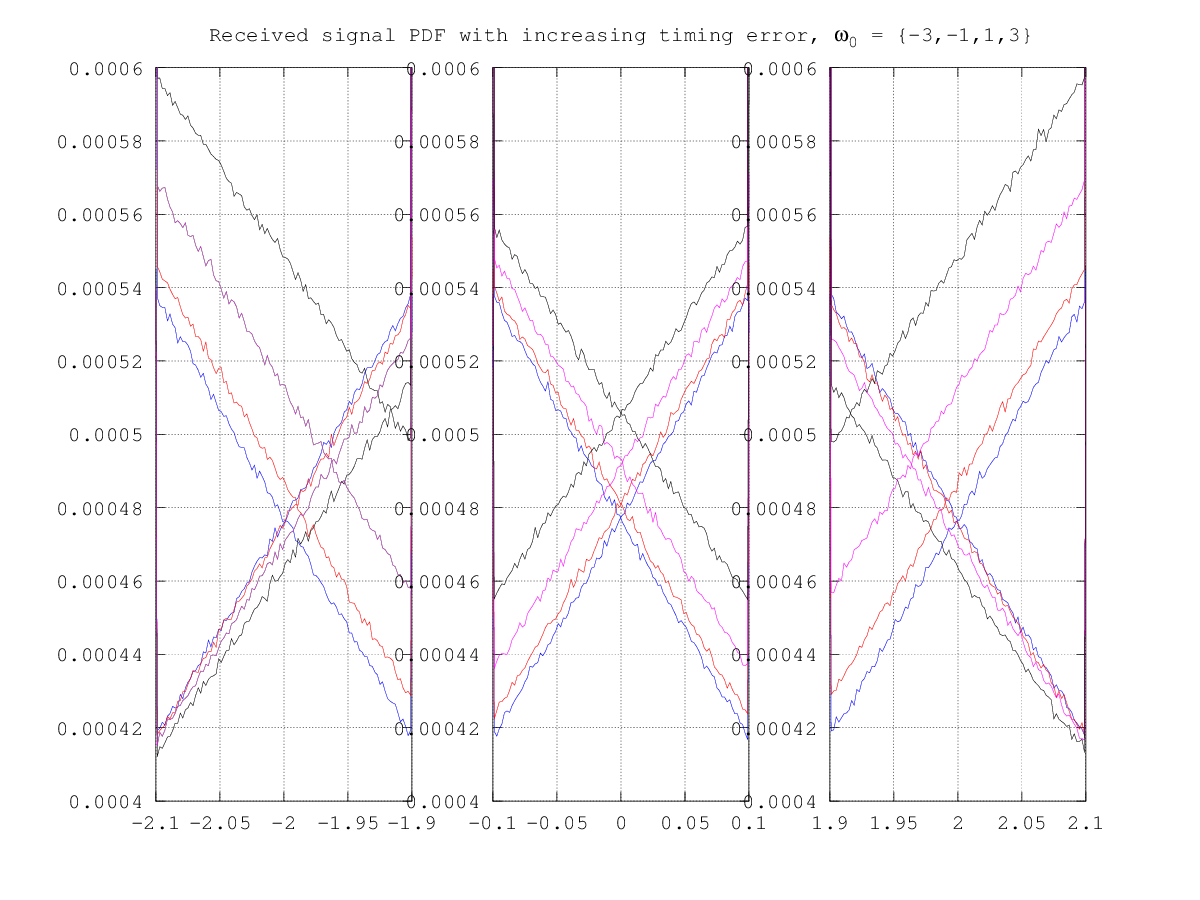
\includegraphics[width=0.8\linewidth]{../../../plots/4pamdecisionerror.png}
\caption[Non-fading received symbol PDF]{Recieved signal PDF for a number of timing offsets (4-PAM, AWGN channel, SNR=4dB))}
\end{figure}

The effects of timing error offset were significant enough to warrant a study using a more realistic fading model, in order to determine the effects in a typical system.

\section{Effects of timing error on the Rayleigh-fading system}

The previous model was extended to include the effects of Rayleigh-distributed fading. The receiver was extended to an l-antenna system, accompanied with selectable EGC or MRC techniques. Timing error was implemented as a Tikhonov-distributed stochastic process.

Both EGC and MRC systems were similarly examined, and in both cases the effects of timing error were also present, to a lesser extent than in the non-fading case, as the antenna diversity has an averaging effect on the received signal. Nonetheless the presence of attenuation suggested that decoding performance was sub-optimal, and could be improved through decoder redesign.

\section{Optimal decoding in the presence of timing error}

The optimum decision region boundaries can be shown to be the intersection between adjacent symbol's PDFs at the input to the decoder. The received symbol histograms generated through simulation were used to determine the optimum decision region boundaries, and the Symol Error Rate defined as the probability of a symbol being incorrectly decoded by the decoder.

\[
\text{SER} = \int\limits_{Y_{DRB}}^{\infty} H_1 (Y) \; dY + \int\limits_{- \infty}^{Y_{DRB}} H_3 (Y) \; dY
\]

If the $\omega = 1, 3$ histograms $H_1$ and $H_3$ have a bin width $\Delta Y$, and a decision region boundary of $Y_{DRB}$ is chosen, where $Y_{DRB} \simeq (n + \frac{1}{2}) \Delta Y$, then the SER was approximated as

\[
\text{SER} \simeq \sum\limits_{i = (n+1) \Delta Y}^{N} H_1 [i] + \sum\limits_{j = 0}^{n \Delta Y} H_3 [j]
\]

The Symbol Error Rates were determined for a range of timing error variances. EGC was found to perform unsatisfactorily at the target SNR of 20dB, so the MRC system was focused on for the continuation of the project.  Timing offset was shown to increase Symbol Error Rates by up to two orders of magnitude\footnote{4-PAM signalling, l=2, SNR=20dB}.

\marginpar{Note on determining the SER: In this project, symmetric 4-PAM signalling was used, so one of the three decision region boundaries is located at 0 and therefore unaffected by timing error. The overall SER presented here is therefore $\sfrac{2}{3}$ that calculated.}With the fall in received signal amplitude comes a fall in optimum decision region boundary. The optimum decision region boundary for the MRC system was found to drop with increasing timing error. Therefore, the traditional system performs sub-optimally. An optimum receiver was designed taking into account the variance of the timing error, and was found to result in a decrease of up to 11\% in SER, for the given number of diversity branches and SNR.

\begin{figure}[htbp]
\centering
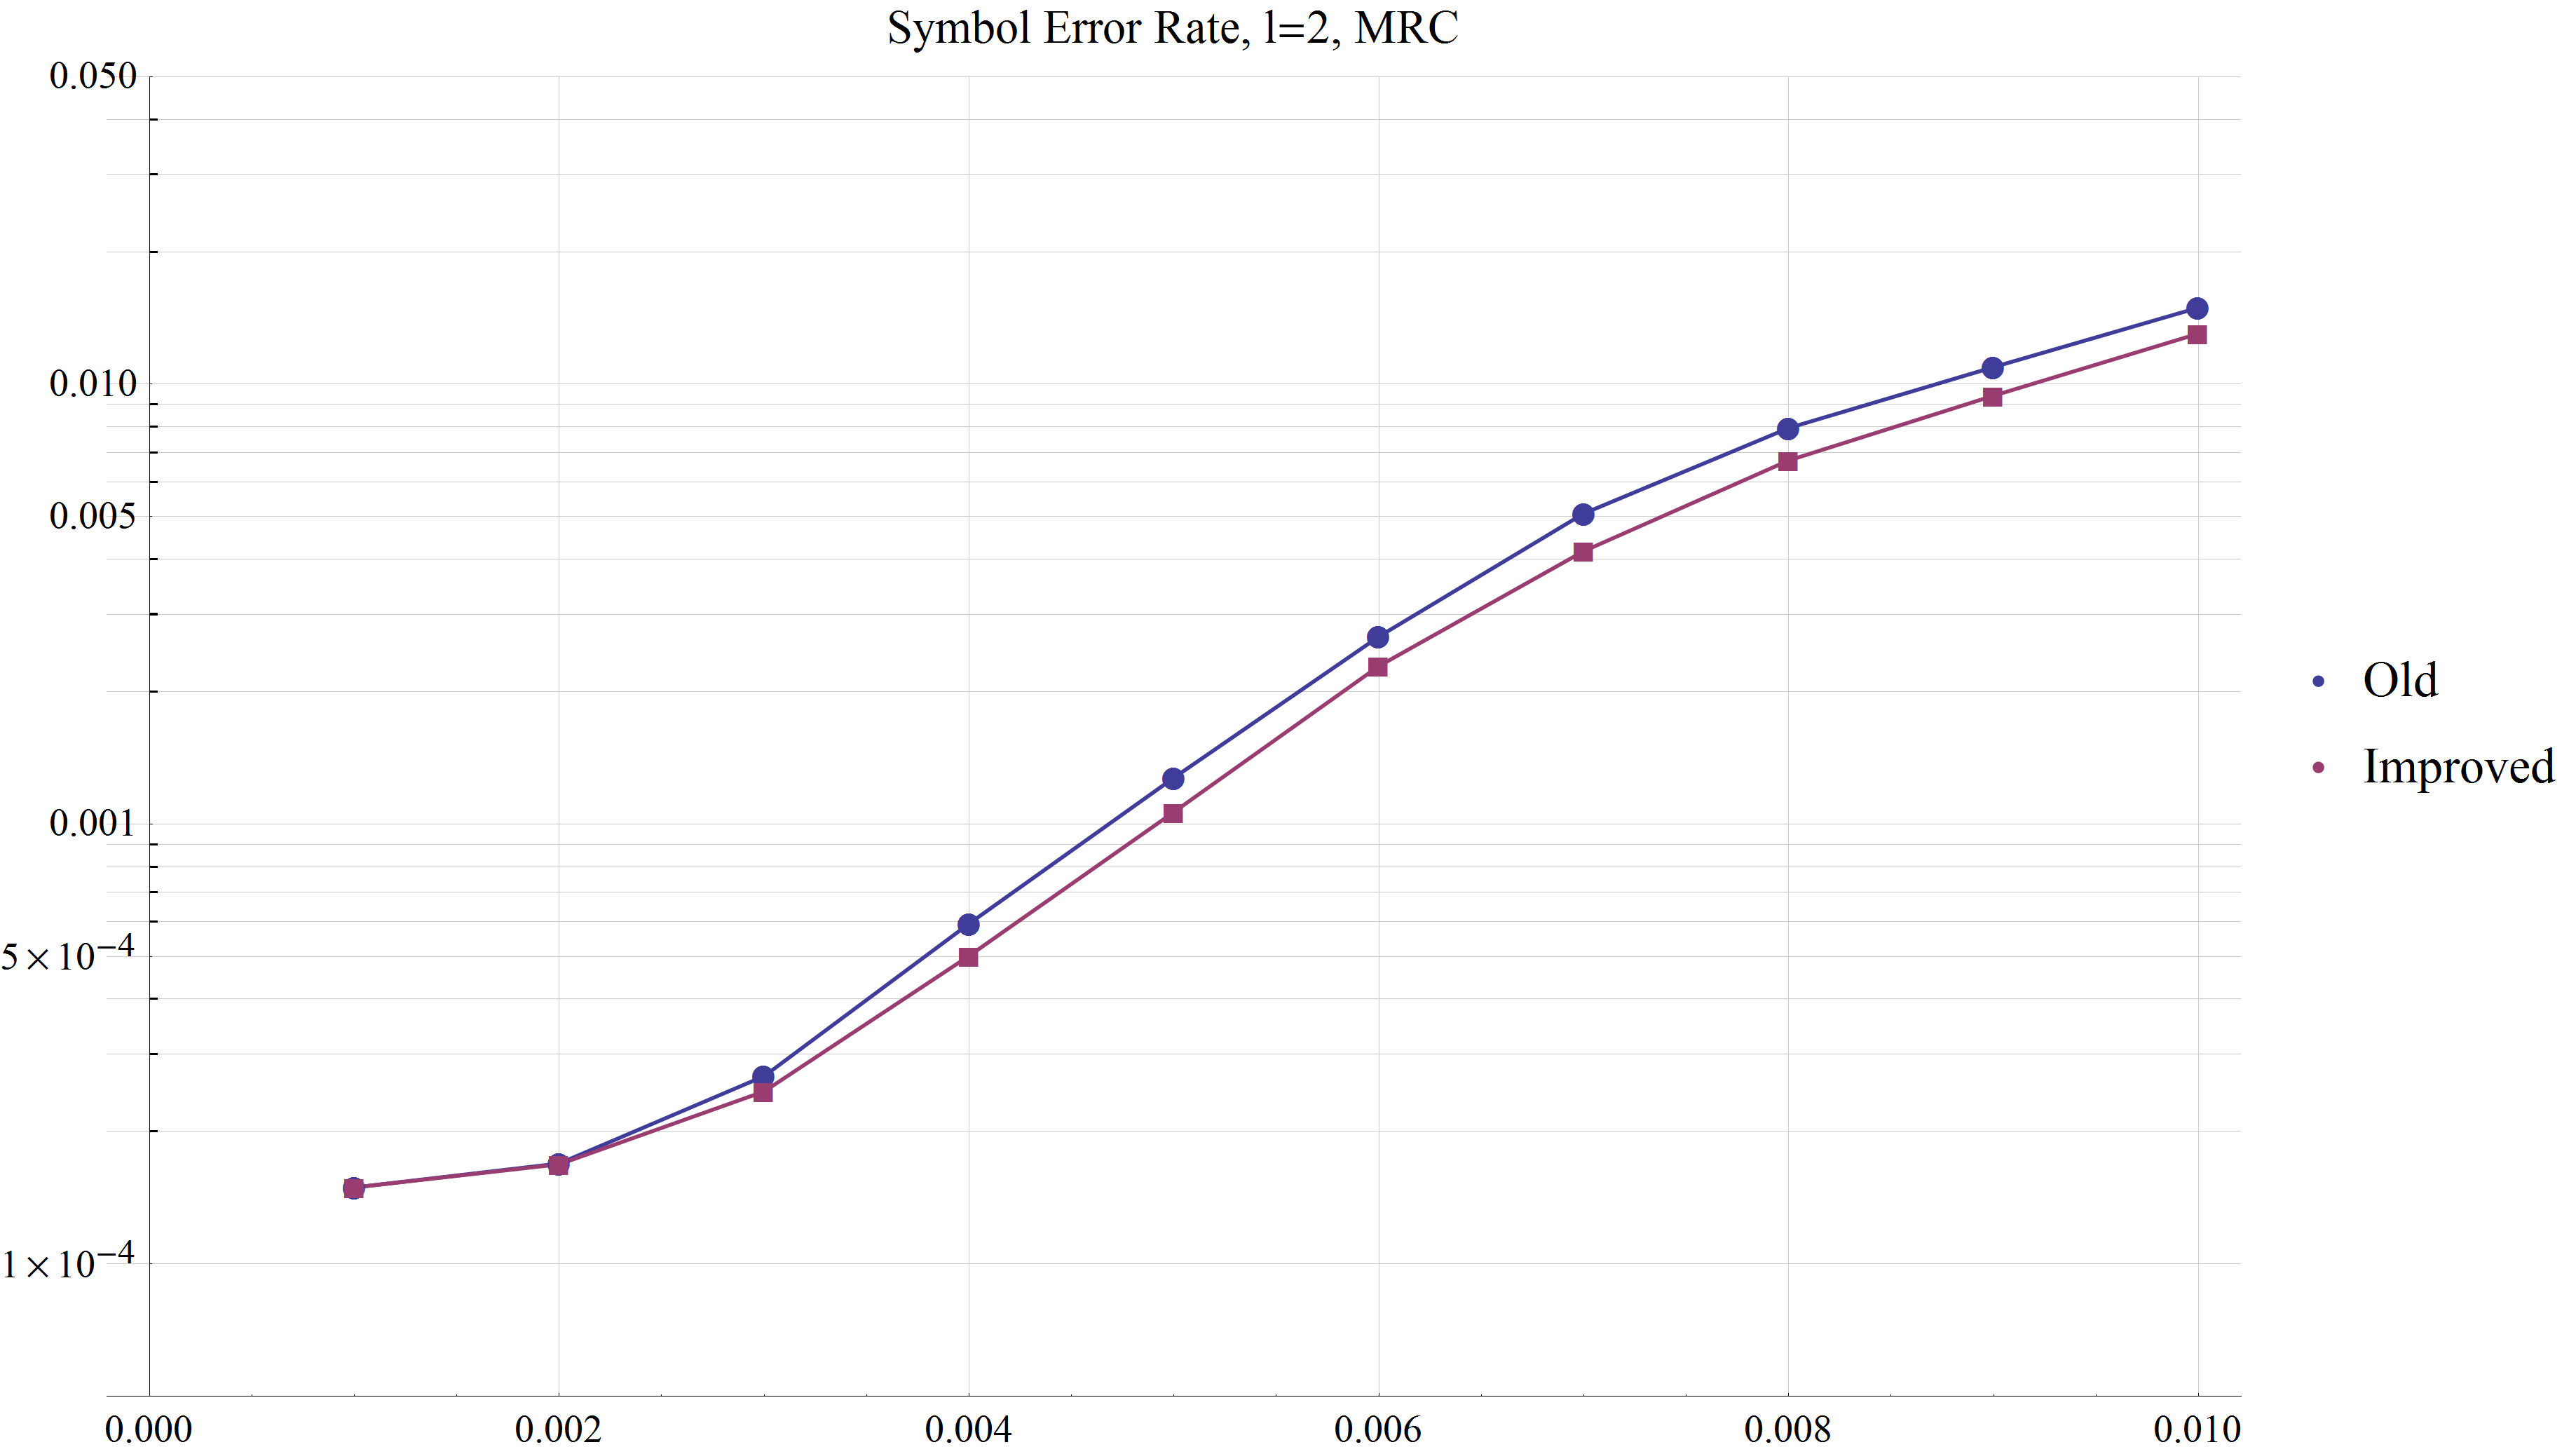
\includegraphics[width=\linewidth]{MRC2_SER.png}
\caption[MRC Symbol Error Rate]{Symbol Error Rate versus timing error variance (4-PAM, Rayleigh-fading AWGN channel, MRC, l=2, SNR=20dB, N= $5 \times 10^{10}$))}
\end{figure}

While the simulation demonstrated the effects of timing error on the described system, a complementary analytical description of the problem would provide additional support to these findings.

\section{Analytical study of timing error}

By approximating the received signal PDF, conditional on set channel gains and timing errors, by a Gram-Charlier series\footnote{See Appendix TODO}, an analytic solution to the conditional PDF was developed. Simulation and analytical plots were compared and the latter was found to be a sufficiently strong approximation to provide an estimate for the optimum decision region boundary.

\begin{figure}[htbp]
\caption[Received signal PDF: Gram-Charlier approximation vs simulation]{Overleaf, left: Comparison between simulated received signal PDF (solid) and Gram-Charlier approximation (dashed)}
\end{figure}

{
\setlength{\floatsep}{2pt plus 1.0pt minus 2.0pt}
\setlength{\textfloatsep}{2pt plus 1.0pt minus 2.0pt}
\setlength{\intextsep}{2pt plus 1.0pt minus 2.0pt}
\begin{figure}[htbp]
\caption[Received signal optimum DRB: Gram-Charlier approximation vs simulation]{Overleaf, right: Comparison between simulated received signal optimum decision region boundary (solid) and Gram-Charlier approximation (dashed)}
\end{figure}
}

\begin{figure}[htbp]
\centering
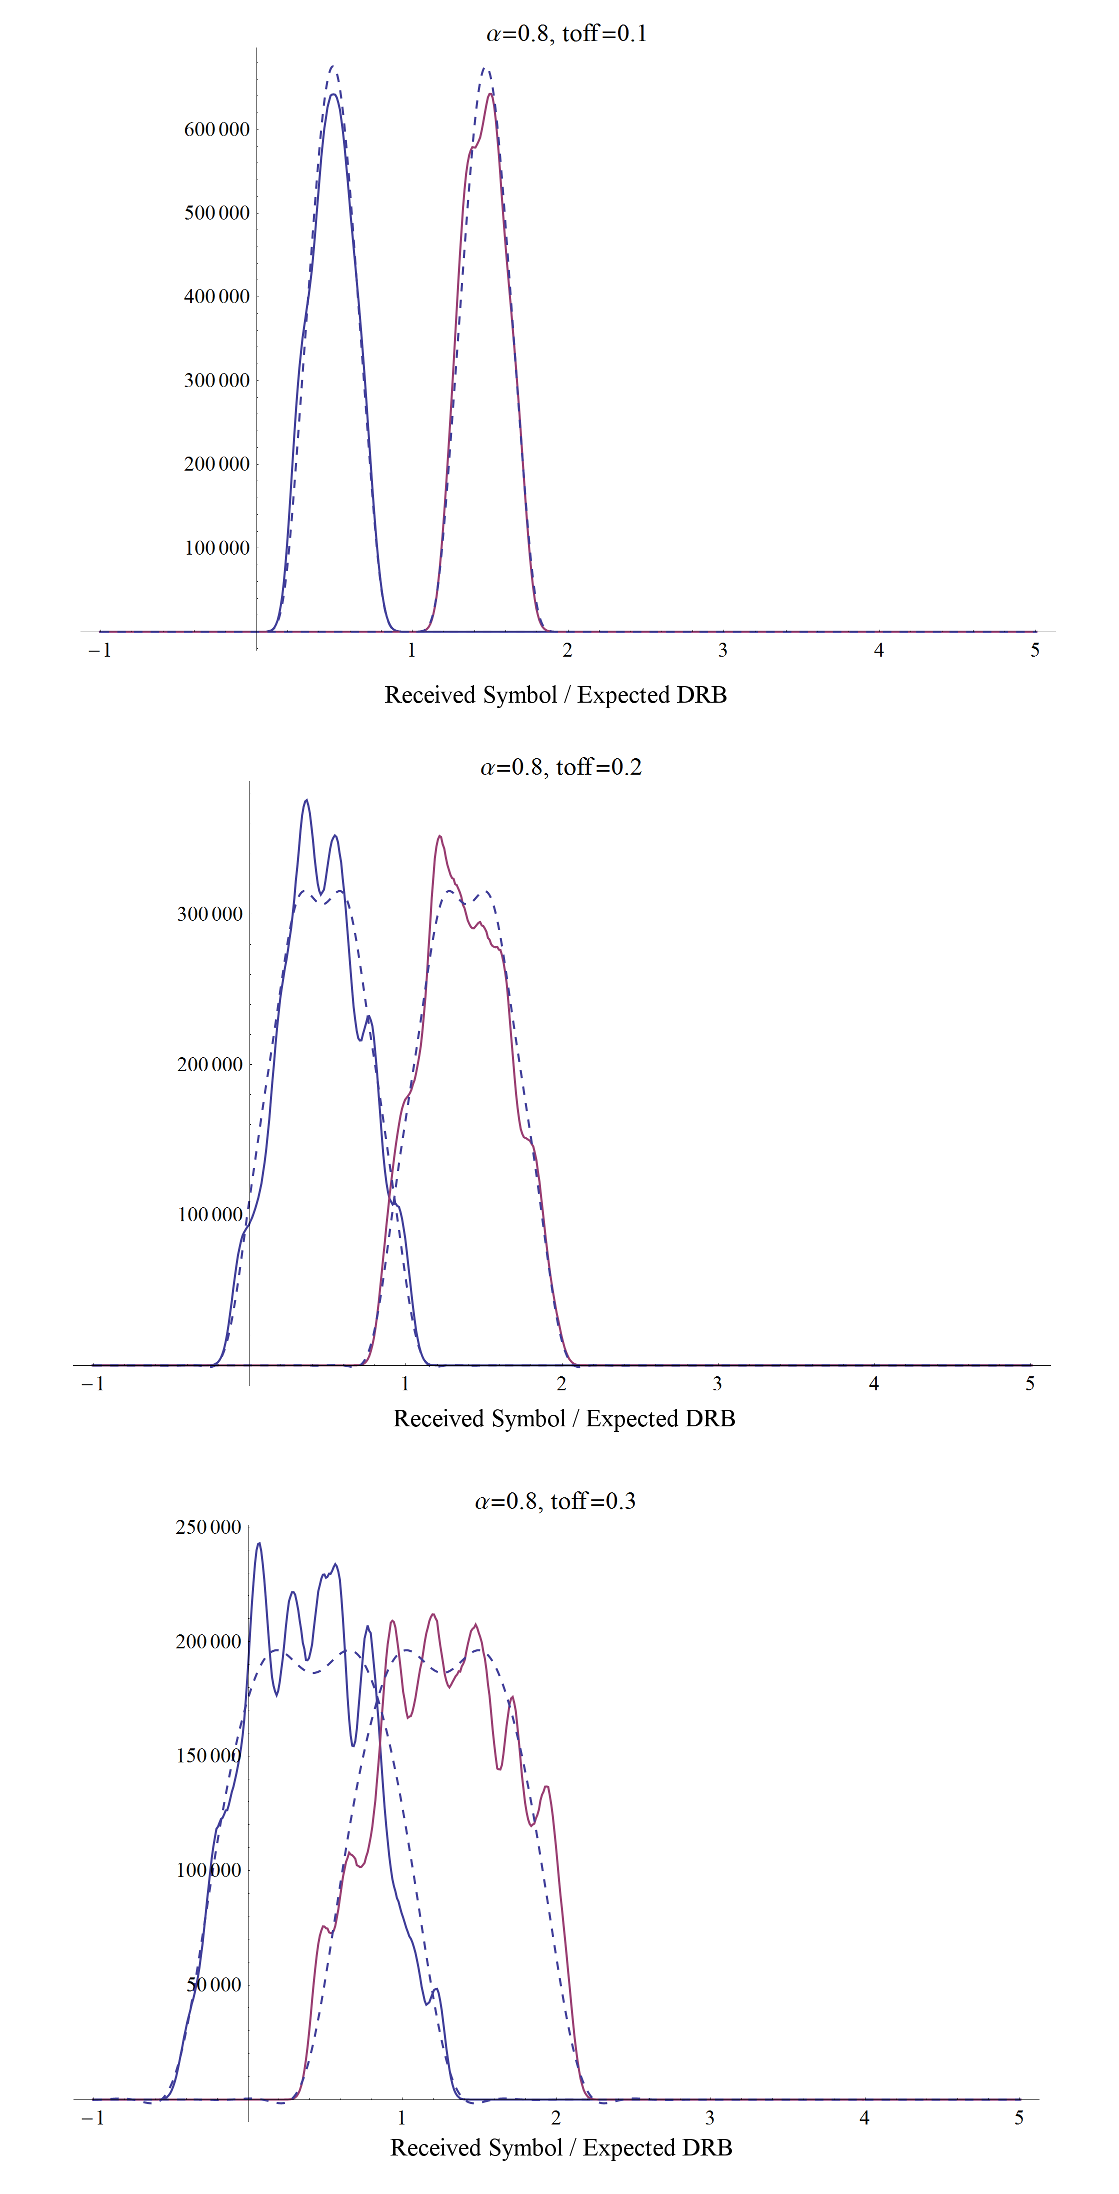
\includegraphics[height=\textheight]{comparison_full.png}
\end{figure}

\begin{figure}[htbp]
\centering
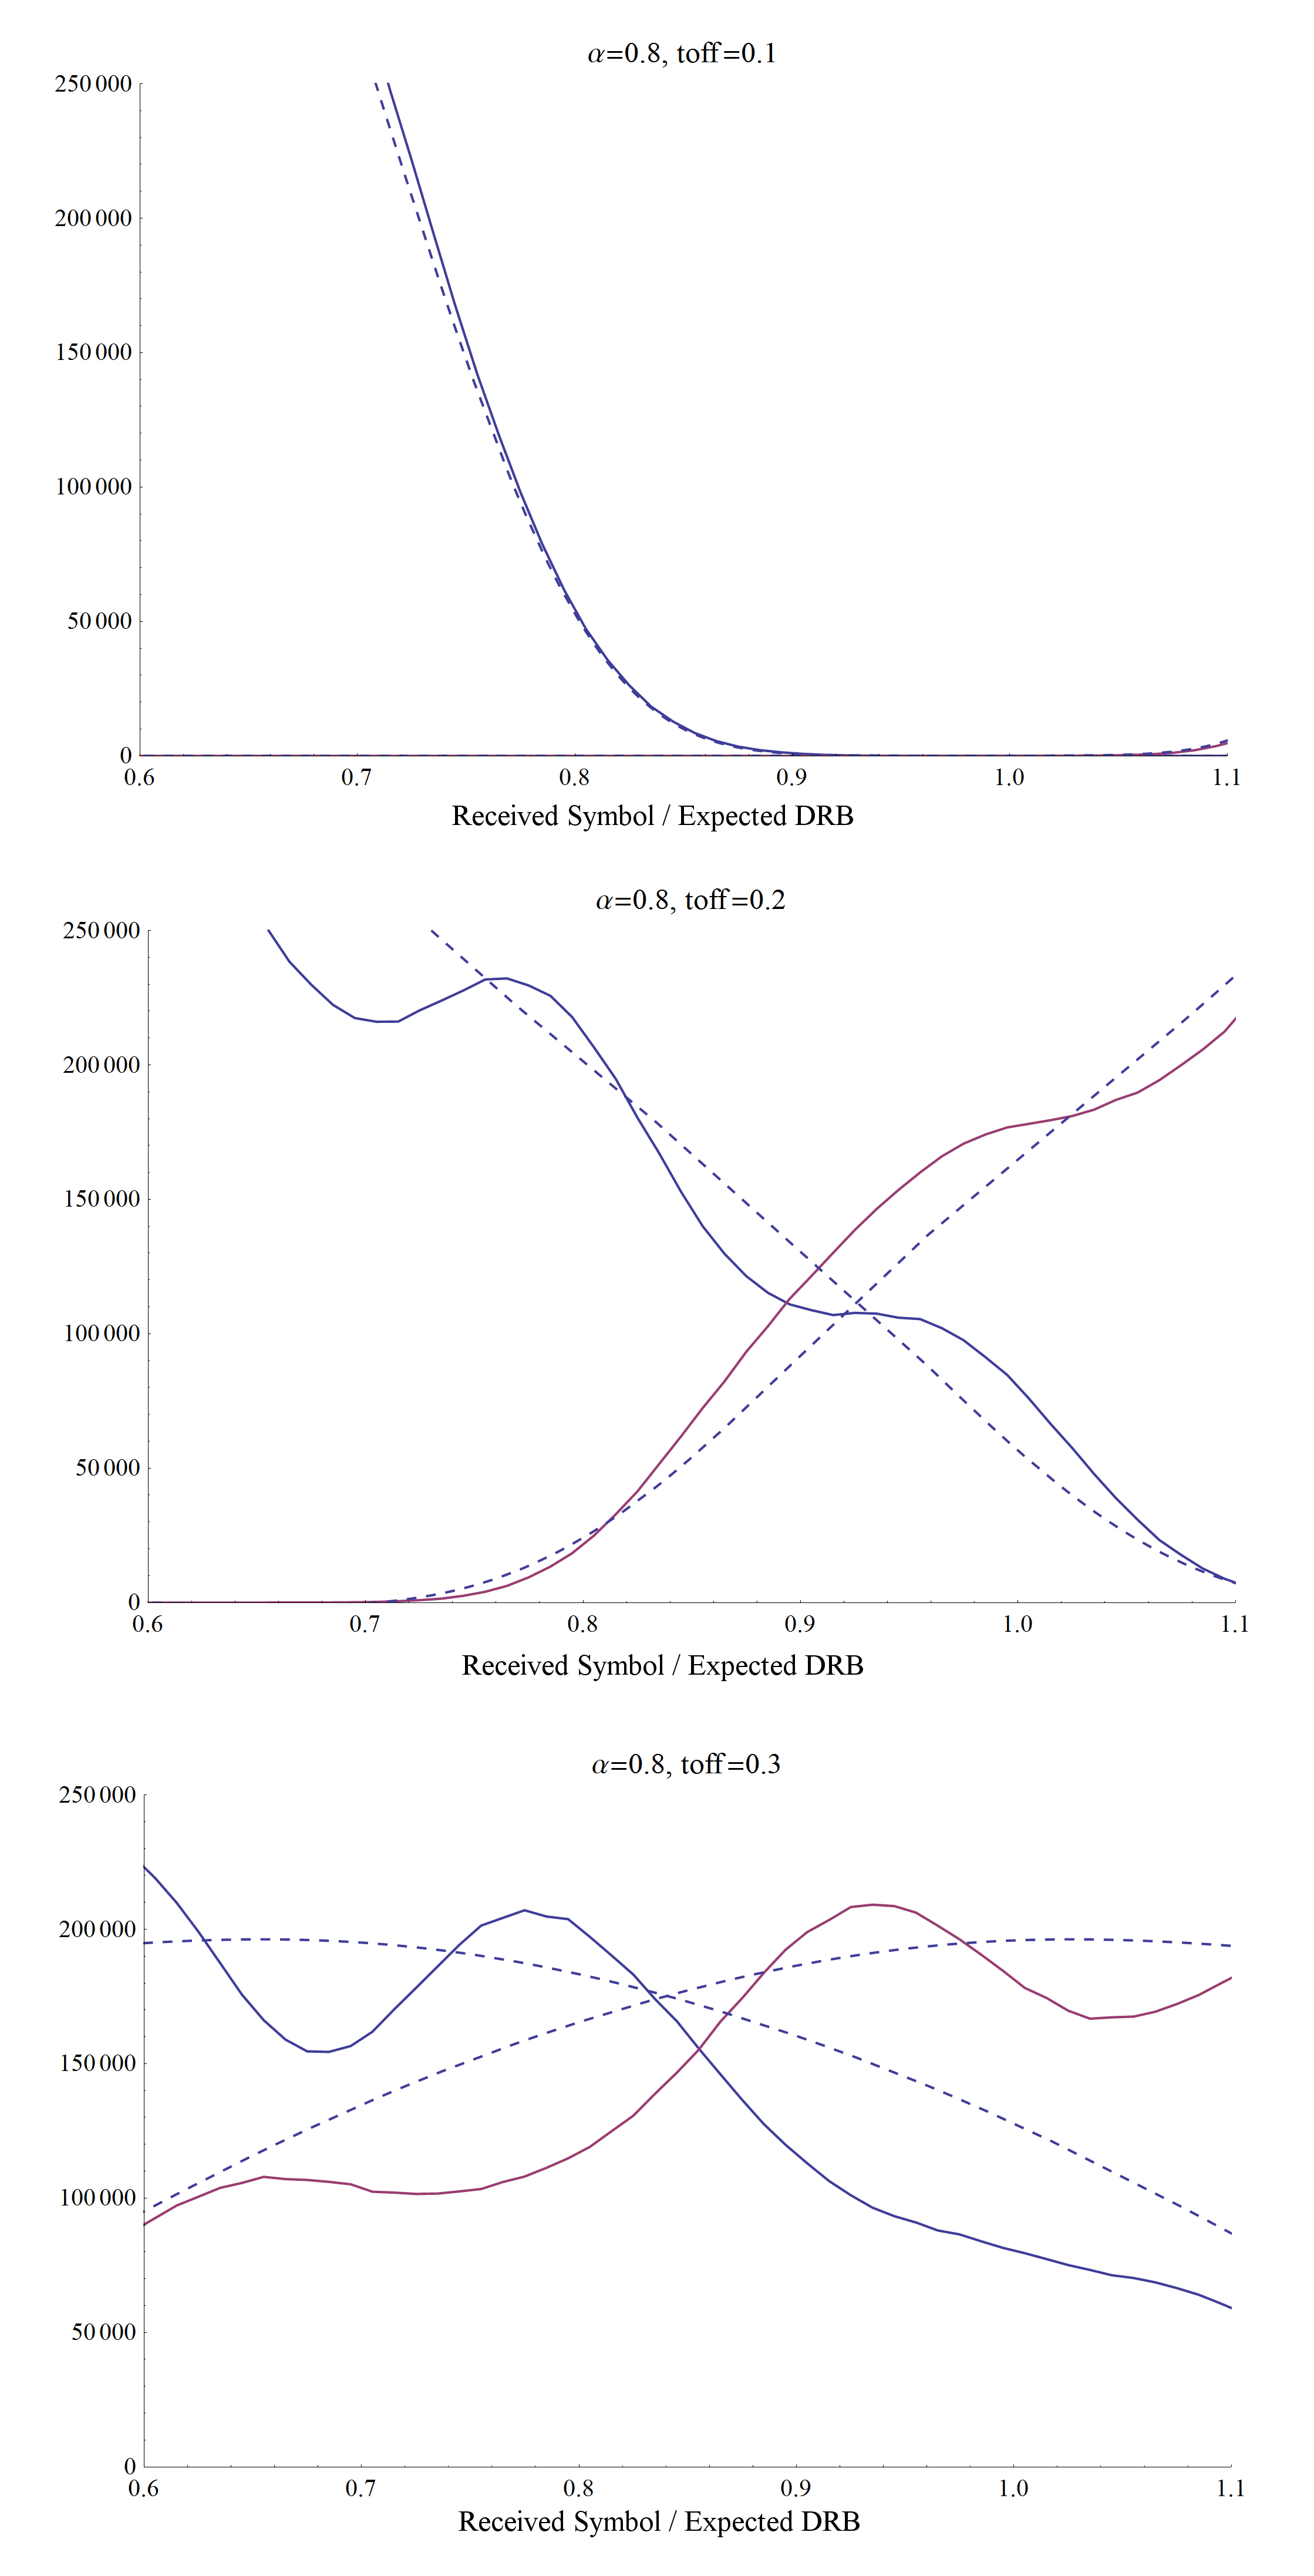
\includegraphics[height=\textheight]{comparison_boundary.png}
\end{figure}

\chapter{Discussion of results}

This project has demonstrated a fundamental effect present to a certain degree in a large number of communications systems. The particular system used to illustrate the problem is representative of a large number of systems; the channel response need not necessarily be Raised-Cosine, merely relatively low-bandwidth, and the effect could occur with any similar choice of fading or timing distribution.

The proposition that the conditional effects of timing error on the received symbol could be approximated by an attenuation was proven through simulation. Furthermore, it was shown that this property could be used to reduce the effects of timing error offset through redesigning the symbol detection algorithm, and the effectiveness of this route was proven.

While the improvements may not seem massive, it is key to note that the change is made \emph{without adding any stages to the detector}. The proposed changes can be implemented with minimum complexity - the factor change in decision region boundary for a given timing error can be pre-determined and stored in a look-up table,  and current timing statistics can be used to address the relevant correction factor.

\begin{figure}[htbp]
\centering
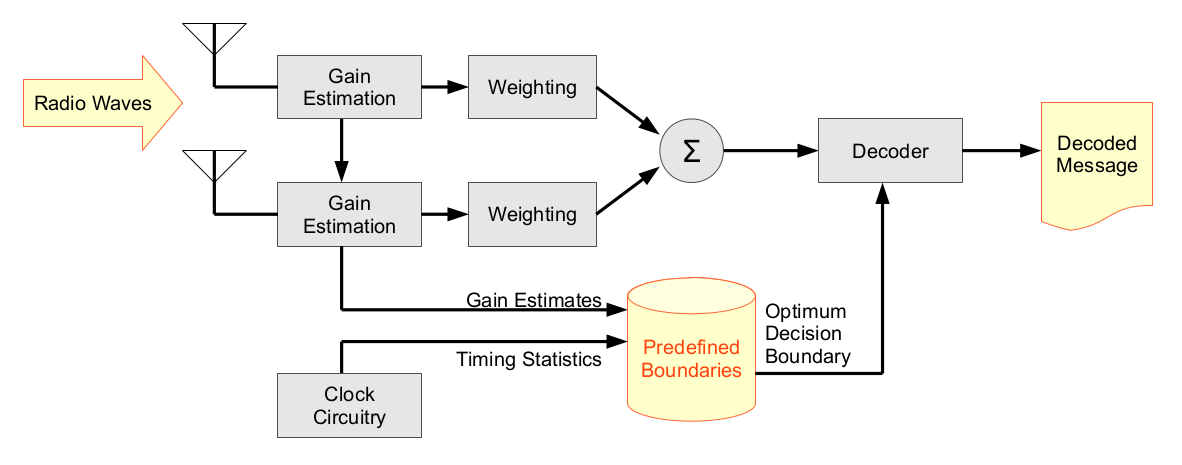
\includegraphics[width=\linewidth]{system.png}
\caption[Improved decoder implementation]{Improved decoder implementing the described corrections as a LUT and multiplier block.}
\end{figure}

\chapter{Future Work}

Future work will be carried out by the author on extending the analytical solution to the conditional PDF to an analytical solution for the overall PDF, with a goal to deriving the optimum decision region boundary for a given timing error variance. This would allow the correction terms for a practical system to be determined without having to perform extensive simulation work.

Given a complete analytical solution for the overall received symbol PDF, it would be possible to generate the optimum decision region boundary conditioned on factors other than timing error variance, such as channel gain and channel SNR. The performance gains from such a system would have to be offset against system cost, but these parameters are readily available to the system.

An extension of the theory presented here to other receiver architectures, channel models and conditions would be a logical continuation to this project, and would help determine the areas in which timing errors are of most concern. In particular, Nakagami-n fading and the effects of increased diversity were not studied, and could yield some interesting results.

This project has theoreticized a fundamental issue present in amplitude-modulated communications systems prone to timing errors. It would be complemented with a practical description of the problem. The described 4-PAM MRC system could be implemented and either the timing offsets artificially added in or the hardware's own timing error monitored.

\chapter{Conclusions}




